\documentclass[12pt,letterpaper]{article}
\usepackage[utf8]{inputenc}
\usepackage[spanish]{babel}
\usepackage{graphicx}
\usepackage[left=2cm,right=2cm,top=2cm,bottom=2cm]{geometry}
\usepackage{graphicx} % figuras
% \usepackage{subfigure} % subfiguras
\usepackage{float} % para usar [H]
\usepackage{amsmath}
%\usepackage{txfonts}
\usepackage{stackrel} 
\usepackage{multirow}
\usepackage{enumerate} % enumerados
\renewcommand{\labelitemi}{$-$}
\renewcommand{\labelitemii}{$\cdot$}
% \author{}
% \title{Caratula}
\begin{document}

% Fancy Header and Footer
% \usepackage{fancyhdr}
% \pagestyle{fancy}
% \cfoot{}
% \rfoot{\thepage}
%

% \usepackage[hidelinks]{hyperref} % CREA HYPERVINCULOS EN INDICE

% \author{}
\title{Caratula}

\begin{titlepage}
\begin{center}
\large{UNIVERSIDAD PRIVADA-DE-TACNA}\\
\vspace*{-0.025in}
\begin{figure}[htb]
\begin{center}

\includegraphics[width=8cm]{./Imagenes/logo}
\end{center}
\end{figure}
\vspace*{0.15in}
INGENIERIA DE SISTEMAS  \\

\vspace*{0.5in}
\begin{large}
TITULO:\\
\end{large}

\vspace*{0.1in}
\begin{Large}
\textbf{INFORME DE LABORATORIO No 04} \\
\end{Large}

\vspace*{0.3in}
\begin{Large}
\textbf{CURSO:} \\
\end{Large}

\vspace*{0.1in}
\begin{large}
BASE DE DATOS II\\
\end{large}

\vspace*{0.3in}
\begin{Large}
\textbf{DOCENTE(ING):} \\
\end{Large}

\vspace*{0.1in}
\begin{large}
 Patrick Cuadros Quiroga\\
\end{large}

\vspace*{0.2in}
\vspace*{0.1in}
\begin{large}
Integrantes: \\
\begin{flushleft}
Arlyn Cotrado Coaquira		\hfill	(2016054466) \\
Yaneth Virginia Aquino Huallpa		\hfill	(2017059286) \\
Sharon Sosa Bedoya            	\hfill	(2016054460) \\
Marlon Villegas Arando	\hfill	(2015053890) \\
\end{flushleft}
\end{large}
\end{center}

\end{titlepage}


\tableofcontents % INDICE
\thispagestyle{empty} % INDICE SIN NUMERO
\newpage
\setcounter{page}{1} % REINICIAR CONTADOR DE PAGINAS DESPUES DEL INDICE

\section{INFORMACIÓN GENERAL} 

\begin{itemize}
\subsection{Objetivos:}
	\item Conocer los fundamentos sobre contenedores y Docker.
	\item Poder instalar correctamente una instancia.
\subsection{Equipos, materiales, programas y recursos utilizados:}
	\item Virtualización activada en el BIOS.
	\item Windows 10 64bit: Pro, Enterprise o Education, con al menos 4GB de RAM.
	\item Docker Desktop
	\item Microsoft SQL Server 2017 o superior

\end{itemize}

\section{MARCO TEORICO} 

\subsection{DOCKER}








\section{PROCEDIMIENTO} 

\begin{itemize}
\subsection{Parte 1: Iniciando Docker}
	\item Abrir el menu inicio y buscar la aplicación Docker for Windows.

	\item Ubicar la aplicación PowerShell, ejecutarla como Administrador. En la ventana de comandos de PowerShell escribir
lo siguiente.
		\begin{figure}[H]
		\begin{center}
		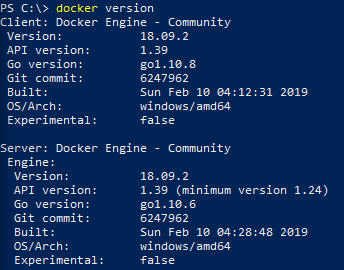
\includegraphics[width=8cm]{./Imagenes/1}
		\end{center}
		\end{figure}
     
\subsection{Parte 2: Creando un contenedor con Oracle Database para Linux}
	\item En un navegador de internet acceder a la dirección https://hub.docker.com/. Iniciar sesión o crear una cuenta nueva
	\item Buscar el repositorio para Oracle Database. Ingresar y proceder con el CheckOut, completar los datos y aceptar las condiciones obligatorias para obtener el acceso al contenido.
		\begin{figure}[H]
		\begin{center}
		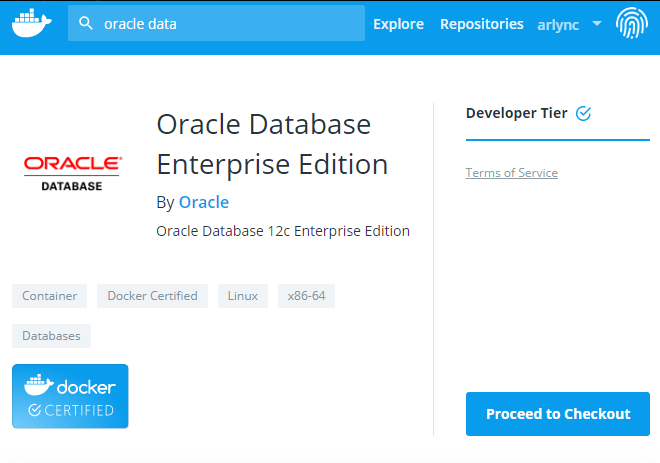
\includegraphics[width=8cm]{./Imagenes/3}
		\end{center}
		\end{figure}
	\item En la ventana de PowerShell, escribir el siguiente comando:
		\begin{figure}[H]
		\begin{center}
		
\includegraphics[width=9cm]{./Imagenes/4}
		\end{center}
		\end{figure}
	\item Ejecutar el siguiente comando en Powershell, lo cual descargará la imagen del contenedor de Oracle Database en un servidor Linux
		\begin{figure}[H]
		\begin{center}
		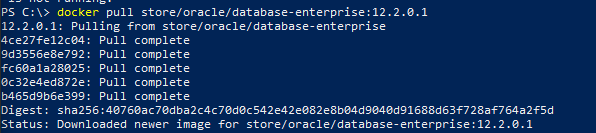
\includegraphics[width=15cm]{./Imagenes/5}
		\end{center}
		\end{figure}
	\item Seguidamente ejecutar el comando, como respuesta se visualizará un ID que corresponde al contenedor.
		\begin{figure}[H]
		\begin{center}
		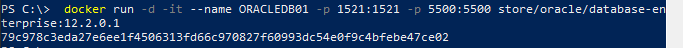
\includegraphics[width=15cm]{./Imagenes/6}
		\end{center}
		\end{figure}
	\item Verificar que el contenedor se esté ejecutando correctamente mediante el comando:
		\begin{figure}[H]
		\begin{center}
		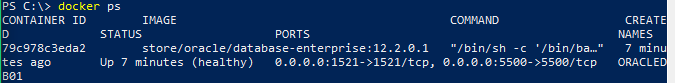
\includegraphics[width=15cm]{./Imagenes/7}
		\end{center}
		\end{figure}
	\item Cuando el estado del contenedor sea “healthy”, en la consola de Powershell, ejecutar el siguiente comando:
		\begin{figure}[H]
		\begin{center}
		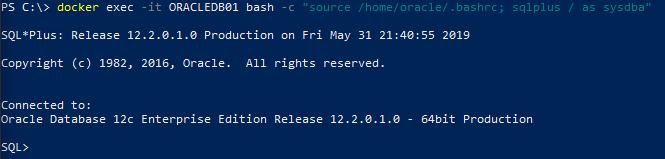
\includegraphics[width=15cm]{./Imagenes/8}
		\end{center}
		\end{figure}
	\item En la línea de comentados de SQL*Plus, escribir lo siguiente
		\begin{figure}[H]
		\begin{center}
		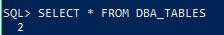
\includegraphics[width=8cm]{./Imagenes/9}
		\end{center}
		\end{figure}
	\item Escribir el comando quit para cerrar la sesión de SQL*Plus
		\begin{figure}[H]
		\begin{center}
		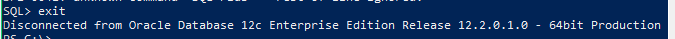
\includegraphics[width=15cm]{./Imagenes/10}
		\end{center}
		\end{figure}
	\item En una pestaña nueva del navegador de internet acceder a la siguiente dirección:https://localhost:5500/em. Iniciar sesión con los siguientes datos:
		\begin{figure}[H]
		\begin{center}
		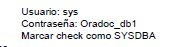
\includegraphics[width=4cm]{./Imagenes/t1}
		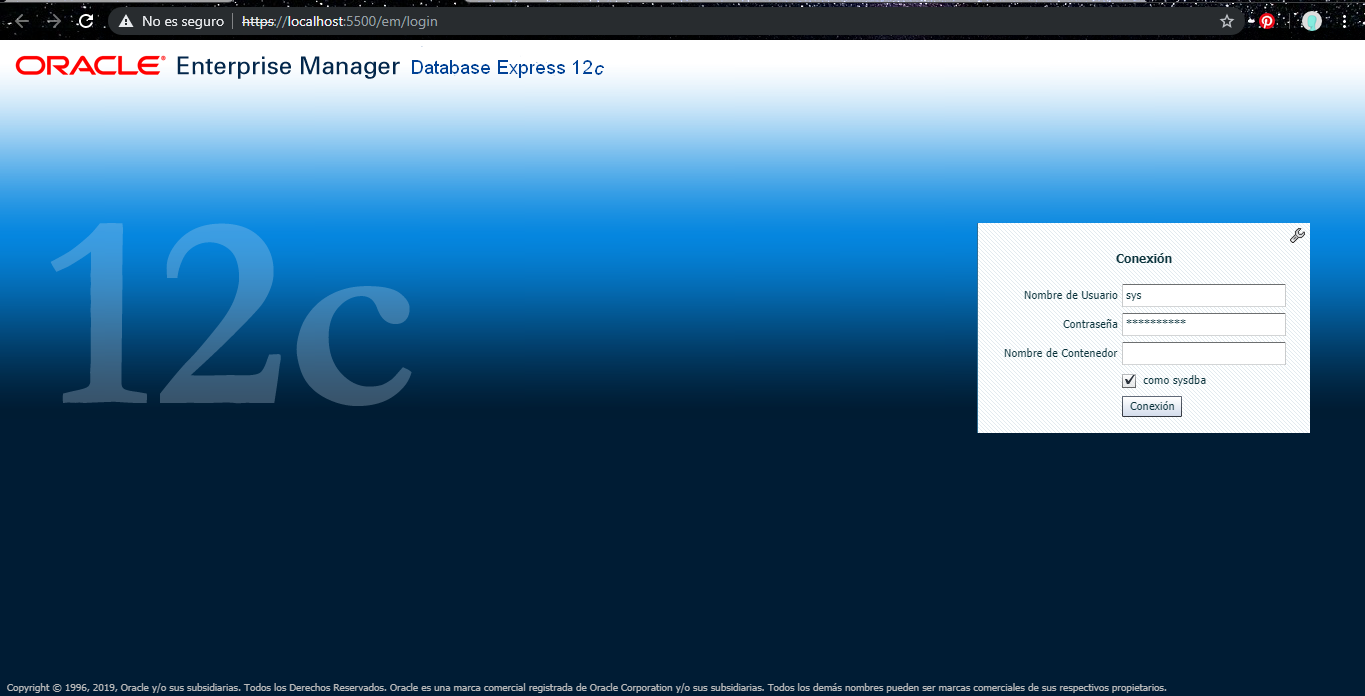
\includegraphics[width=15cm]{./Imagenes/11}
		\end{center}
		\end{figure}
	\item Luego se visualizará la siguiente ventana. Cerrar sesión y la pestaña del navegador de internet.
		\begin{figure}[H]
		\begin{center}
		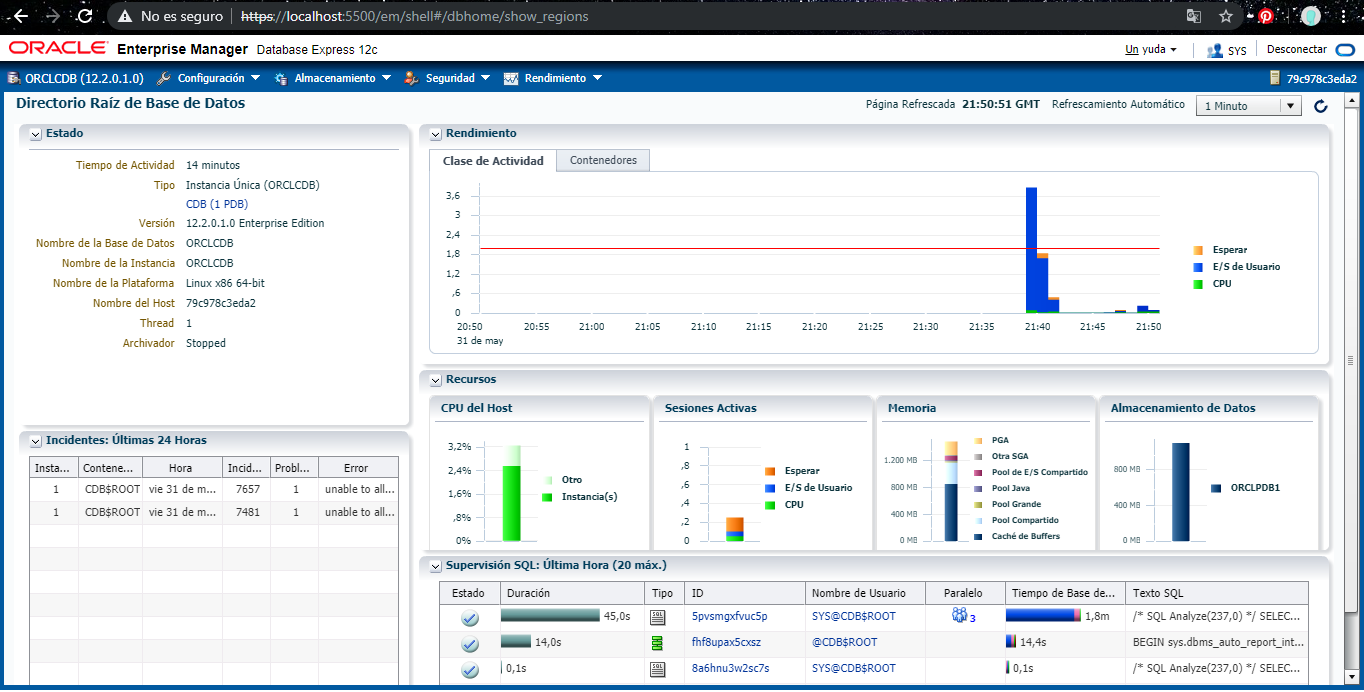
\includegraphics[width=15cm]{./Imagenes/12}
		\end{center}
		\end{figure}
	\item Iniciar el aplicativo Oracle SQL Developer, crear una nueva conexión con los siguientes parámetros:
		\begin{figure}[H]
		\begin{center}
		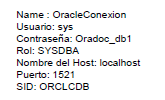
\includegraphics[width=5cm]{./Imagenes/t2}
		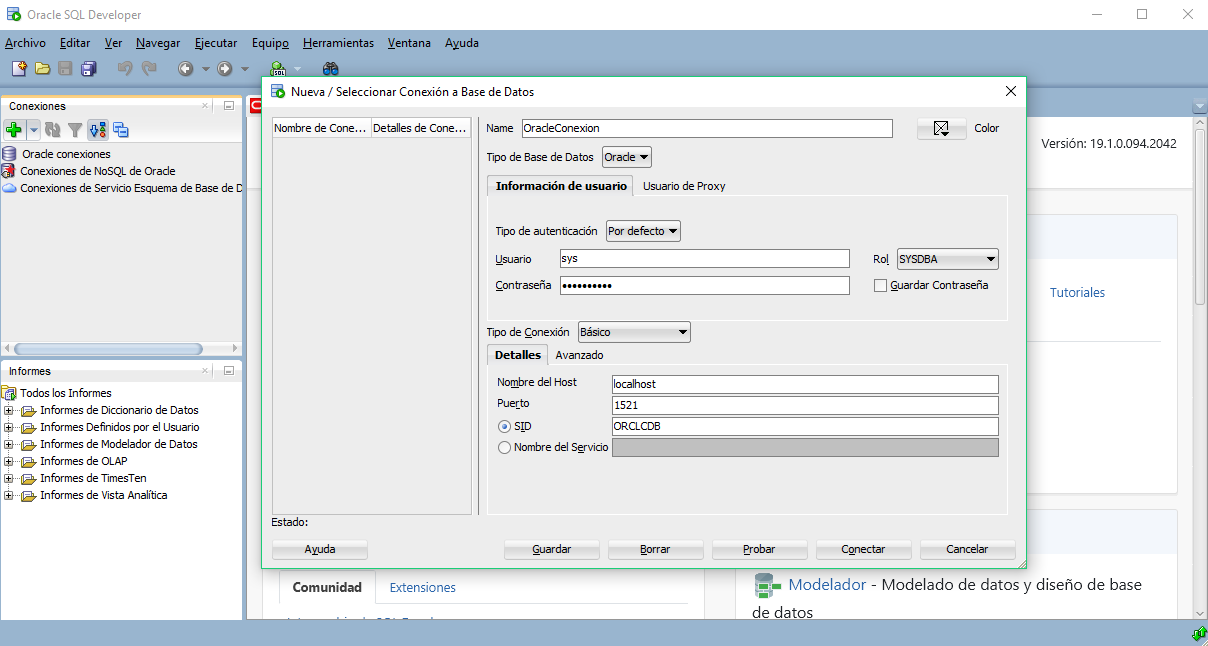
\includegraphics[width=15cm]{./Imagenes/13}
		\end{center}
		\end{figure}
	\item Iniciar una nueva consulta, escribir y ejecutar lo siguiente; deberá retornar varios registros que representan las tablas de las base de datos
		\begin{figure}[H]
		\begin{center}
		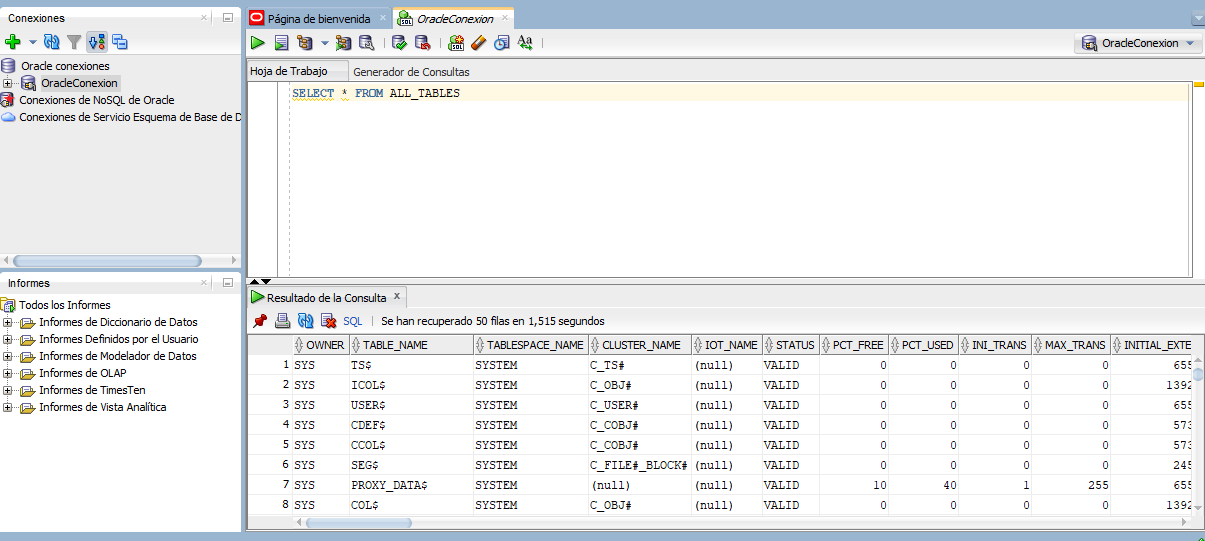
\includegraphics[width=15cm]{./Imagenes/14}
		\end{center}
		\end{figure}
	\item Cerrar la aplicación Oracle SQL Developer
	\item En PowerShell ejecutar el siguiente comando. Y verificar la eliminación del contenedor con ejecutando
		\begin{figure}[H]
		\begin{center}
		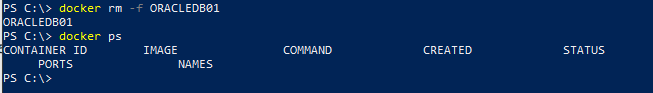
\includegraphics[width=12cm]{./Imagenes/15}
		\end{center}
		\end{figure}


\subsection{Parte 3: Adicionando persistencia}
	\item Abrir el menu inicio y buscar la aplicación Docker for Windows.
       
\end{itemize}
		
\section{ANALISIS E INTERPRETACION DE RESULTADOS} 


\subsection{Parte 1: Actividades Encargadas}
	\begin{itemize}
		\item ¿Con qué comando(s) puedo iniciar y detener una instancia de Oracle, detalle cada uno de los pasos y opciones,
utilizando Docker?
                     \item Para  Iniciar una instancia de Oracle Database Server
Iniciar una instancia de servidor de base de datos Oracle al ejecutar
" docker run -d -it --name oracle-db store/oracle/database-enterprise:12.2.0.1"donde oracle01-db está el nombre del contenedor y 12.2.0.1 es la etiqueta de imagen de Docker.
                      \begin{figure}[H]
		\begin{center}
		
\includegraphics[width=15cm]{./Imagenes/200}
		\end{center}
		\end{figure}
                      \item Los comandos docker ps -a -q detendrá todos los contenedores Docker en ejecución :
                      \begin{figure}[H]
		\begin{center}
		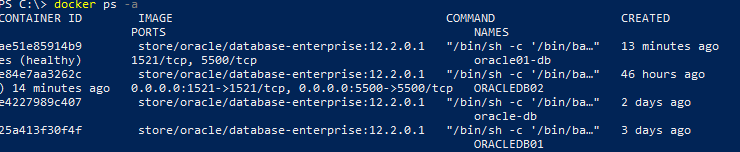
\includegraphics[width=15cm]{./Imagenes/201}
                      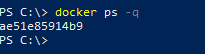
\includegraphics[width=8cm]{./Imagenes/202}
		\end{center}
		\end{figure}
		\item ¿Con qué comando(s) puedo iniciar y detener el Listener y el Enterprise manager, detalle cada uno de los pasos y
opciones, utilizando Docker?
		\item Genere un nuevo contenedor y cree un espacio de tablas con las siguientes características.
		\begin{figure}[H]
		\begin{center}
		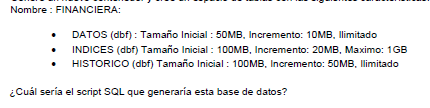
\includegraphics[width=8cm]{./Imagenes/t3}
		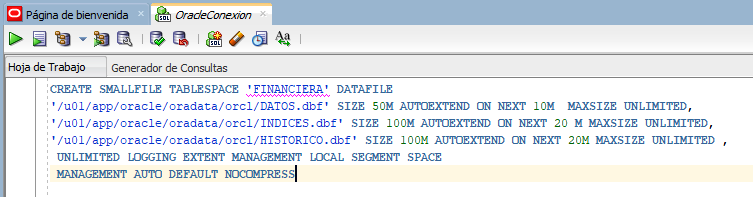
\includegraphics[width=15cm]{./Imagenes/23}
		\end{center}
		\end{figure}


	\end{itemize}




\section{CONCLUSIONES}
Como podemos apreciar, hoy tenemos una tecnología disponible desde hace unos años que nos permite ir a otro nivel de virtualización distinto, permitiéndonos obtener las siguientes ventajas:
\begin{itemize}
\item Instalación simple y capacidad de ejecutar múltiples aplicaciones en entornos aislados sobre un mismo sistema operativo,  permitiéndonos ahorrar horas de trabajo en la administración de Infraestructura.
\item Independiente a la plataforma, permite contar con soluciones más portables.
\item Despliegue de Aplicaciones mucho más rápida y flexible.
\item Disponible en múltiples proveedores de Nube.
	
\end{itemize}

\newpage

\section{REFERENCIAS} 

\begin{itemize}
	\item [[ 1]] Hat, R. (2017). ¿Qué es Docker?. Recuperado de https://www.redhat.com/es/topics/containers/what-is-docker
	
\end{itemize}




\end{document}
